\documentclass[tikz,border=2pt]{standalone}
\usepackage{amsmath}
\usepackage{pgfplots}
\pgfplotsset{compat=1.18}
\usetikzlibrary{arrows.meta,decorations.pathreplacing}
\begin{document}
% The four atomic types used in the course, with an example value and what typeof() and class()
% return; is.numeric() is TRUE for double and integer.
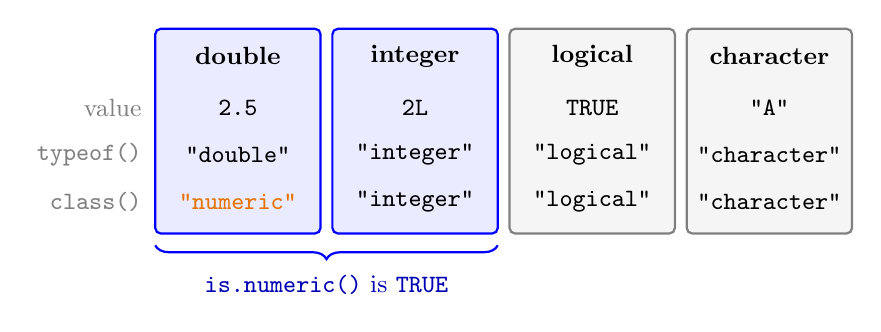
\begin{tikzpicture}[font=\small, >={Latex[length=2mm]}]
  \foreach \i/\name/\val/\tp/\cl/\col in {
      0/double/2.5/"double"/"numeric"/blue,
      1/integer/2L/"integer"/"integer"/blue,
      2/logical/TRUE/"logical"/"logical"/gray,
      3/character/"A"/"character"/"character"/gray} {
    \pgfmathsetmacro{\x}{1.6+2.25*\i}
    \draw[\col, thick, rounded corners=2pt, fill=\col!8] (\x-1.05,0) rectangle (\x+1.05,2.6);
    \node[font=\small\bfseries] at (\x,2.25) {\name};
    \node[font=\small\ttfamily] at (\x,1.6) {\val};
    \node[font=\small\ttfamily] at (\x,1.0) {\tp};
  }
  \node[font=\small\ttfamily, orange!90!black] at (1.6,0.4) {"numeric"};
  \node[font=\small\ttfamily] at (3.85,0.4) {"integer"};
  \node[font=\small\ttfamily] at (6.1,0.4) {"logical"};
  \node[font=\small\ttfamily] at (8.35,0.4) {"character"};
  \node[anchor=east, gray] at (0.5,1.6) {value};
  \node[anchor=east, gray] at (0.5,1.0) {\texttt{typeof()}};
  \node[anchor=east, gray] at (0.5,0.4) {\texttt{class()}};
  \draw[decorate, decoration={brace, mirror, amplitude=5pt}, thick, blue] (0.55,-0.15) -- (4.9,-0.15);
  \node[blue!70!black] at (2.725,-0.65) {\texttt{is.numeric()} is \texttt{TRUE}};
\end{tikzpicture}
\end{document}
